\chapter{Implementace}
\section{Solr}
Základní komponentou, kterou bylo třeba implementovat, byl Solr. Potřebuji aby software zvládl indexovat text v~českém jazyce. Solr obsahuje předinstalovanou a~částečně předkonfigurovanou českou sadu analyzérů, která zahrnuje \emph{StandardTokenizer}, \emph{LowerCaseFilter}, \emph{StopFilter} a~\emph{CzechStemFilter}. V~tomto pořadí.

\emph{StandardTokenizer} dělí text na tokeny. Po zběžné zkoušce jsem usoudil, že jeho algoritmus je funkční i~pro český jazyk. \emph{LowerCaseFilter} je určen k~převodu textu na malá písmena. I~tento filtr jsem otestoval a~opět se neprojevily žádné problémy --- převádí na malá písmena i~speciální české znaky s~interpunkcí. 

\emph{StopFilter} odebírá tokeny odpovídající slovům v seznamu. Jeho fungování tedy závisí na kvalitě seznamu. V~Solru je předinstalován seznam \\\emph{czech\_stopwords.txt}, jenž obsahuje slova, která jsou v~českém jazyce natolik frekventovaná, že nevypoví o~vyhledávaném textu žádnou zásadní informaci. Jedná se především o~nejrůznější předložky, spojky a~pomocná slovesa. Tento seznam jsem shledal dostačujícím, už proto, že kdykoliv v~případě potřeby půjde seznam rozšířit o~další slova, která se vyskytují příliš často v~policejním prostředí, a~nepomáhají tudíž specifikovat hledaný text.

Poslední \emph{CzechStemFilter} je klíčový analyzér. Jak jsem již psal v~kapitole \ref{analysis}~Analýza, měl by být výsledkem práce švýcarských programátorů. O~jeho kvalitách nejsem zcela přesvědčen, implementoval jsem proto do Solru další české stemmery.

\subsection{Stemmery}
K~tomu, aby mohl být implementovaný \emph{StemFilter} použit v~Solru, je nutno vytvořit JAR knihovnu obsahující třídu implementující rozhraní \emph{TokenFilter} a~zároveň její tovární třídu, nejlépe potomka \emph{TokenFilterFactory}. Sestavená JAR knihovna se pak umístí do adresáře \emph{Lib}, kde z~ní bude moci \emph{ClassLoader} Solru číst. V~konfiguraci Solru je pak již možné použít nový filtr definovaný absolutním jménem tovární třídy. Parametry definované v~konfiguraci se předávají tovární třídě, je tedy možné konfigurací ovlivnit funkci stemmeru.

\subsubsection{Light a~Agressive stemmer}
Vnitřní \emph{CzechStemFilter} Solru je dle dokumentace\cite{sorl:doc} jedním ze stemizačních algoritmů autorů L.~Dolamica a~J.~Savoye. Výsledkem jejich práce\cite{Dolamic:2009:Stemming} je stemizační algoritmus, který je založen na technice postupného hledání a~odtrhávání koncovek slov. Vytvořili dvě verze svého algoritmu, takzvanou light a~agressive verzi, které se liší počtem odebíraných koncovek slov (agresivní verze jich odebírá více). Ani jedna z~těchto verzí ale prostým porovnáním kódu neodpovídá českému filtru implementovanému v~Solru. Rozhodl jsem se proto, že doimplementuji light i~agressive stemmer.

Zdrojový kód obou stemmerů je k~dispozici na internetu v~jazyce Java pod BSD licencí. Jde o~dvě třídy s~implementací. Vytvořil jsem tedy vlastní třídu \emph{CzechStemFilter}, která bude tvořit adaptér implementačním třídám. Dále jsem vytvořil tovární třídu \emph{CzechStemFilterFactory}, která inicializuje \emph{CzechStemFilter} a~dle parametrů v~konfiguraci zvolí \uv{agresivní} či \uv{odlehčenou} implementaci stemmeru. Při tvorbě těchto dvou tříd jsem se inspiroval původní implementací \emph{CzechStemFilter} v~aplikaci Solr.

Výslednou implementaci jsem zkompiloval do knihovny \emph{Analyzery.jar} a~podle výše popsaného postupu integroval do Solru.

\subsubsection{Helebrand stemmer}
V rámci dalšího výzkumu jsem nalezl diplomovou práci D.~Helebranda z~VUT v~Brně\cite{Helebrand:2010:Stemming}, který implementoval stemmer pro český jazyk v~prostředí Snowball. Snowball je programovací jazyk speciálně navržený pro zpracovávání textových řetězců, především právě pro tvorbu stemizačních algoritmů. Výsledný algoritmus lze pomocí nástrojů Snowballu přímo přeložit do jazyka C či Java. Hotový stemizační algoritmus pana Helebranda je k~dispozici pod licencí GNU General Public License.

Získal jsem tedy algoritmus z~webových stránek brněnské technické univerzity a~pomocí výše zmíněných nástrojů jsem jej nechal přeložit do Javy. Solr v~sobě již má implementovány stemmery pro několik jazyků pomocí prostředí Snowball, nebylo proto příliš složité výsledný Java algoritmus integrovat. Obsažená tovární třída \emph{SnowballPorterFilterFactory} je příhodně navržená tak, že jméno  portované třídy s~algoritmem hledá v~balíčku \emph{org.tartarus.snowball.ext}. Stačilo tedy jen vygenerovanou třídu s~algoritmem vhodně pojmenovat a~umístit do správného balíčku. \emph{SnowballPorterFilterFactory} přijímá jméno třídy, kterou má hledat, jako parametr z~konfigurace.

Výslednou sestavu jsem přibalil do JAR knihovny s~předchozími implementacemi stemmerů, bude tedy umístěna v~adresáři \emph{Lib}, kde ji \emph{ClassLoader} Solru nalezne.

\subsubsection{Hunspell stemmer}
Po implementaci tří stemmerů založených na postupném odtrhávání koncovek jsem začal hledat řešení, které by používalo jinou metodu získávání kořenů. Hledal jsem algoritmus založený buď na strojovém učení, nebo na porovnávání se slovníkem a~zjistil jsem, že existuje algoritmus, který využívá Hunspell k~odebrání koncovek s~využitím slovníku, a~že je již implementovaný v~Solru.

Hunspell je open source knihovna sloužící ke kontrole pravopisu. Je využívaný například v~projektech Apache OpenOffice či Google Chrome. Slovníky, včetně českého, lze pro Hunspell volně stáhnout přímo z~internetových stránek OpenOffice\cite{openoffice}. České slovníky jsou licencovány pod GNU/GPL licencí. Byly tvořeny pro starší knihovnu Ispell, Hunspell je s~ní však zpětně kompatibilní.

Ze sady souborů českého slovníku v~projektu využiji jen dva: soubor s~koncovkou \emph{.dic}, který obsahuje seznam slov daného jazyka, ideálně v~kořenovém tvaru, a~soubor \emph{.aff}, který obsahuje pravila přidávání koncovek\cite{zdrojak}. Soubor \emph{cs\_CZ.aff} českého slovníku obsahuje syntaktickou chybu, kterou jsem musel před použitím slovníku opravit, protože jinak se Solr při jeho \uv{parsování} ukončí kritickou chybou.

Nevýhodu této metody vidím především v~nedostatečné kvalitě slovníku. Poslední verze pochází z~roku 2008 a~nezdá se, že by byl nadále aktivně rozšiřován.

\subsection{Konfigurace} \label{sorlconfig}
\subsubsection{Datová pole}
K již existujícímu textovému datovému typu \emph{text\_cz}, který používá vestavěný český stemmer, jsem v~konfiguračním souboru \emph{schema.xml} vytvořil datové typy, jenž využívají nově vytvořené stemmery. Toho jsem docílil následující konfigurací.

\begin{verbatim}
<!-- Czech original -->
<fieldType name="text_cz" 
           class="solr.TextField" 
           positionIncrementGap="100">
  <analyzer> 
    <tokenizer class="solr.StandardTokenizerFactory"/>
    <filter class="solr.LowerCaseFilterFactory"/>
    <filter class="solr.StopFilterFactory" 
            ignoreCase="true" 
            words="lang/stopwords_cz.txt" />
    <filter class="solr.CzechStemFilterFactory"/>       
  </analyzer>
</fieldType>

<!-- Czech Helebrand -->
<fieldType name="text_cz_helebrand" 
           class="solr.TextField" 
           positionIncrementGap="100">
  <analyzer> 
    <tokenizer class="solr.StandardTokenizerFactory"/>
    <filter class="solr.LowerCaseFilterFactory"/>
    <filter class="solr.StopFilterFactory" 
            ignoreCase="true" 
            words="lang/stopwords_cz.txt" />
    <filter class="solr.SnowballPorterFilterFactory" 
            language="CzechHelebrand" />       
  </analyzer>
</fieldType>

<!-- Czech Dolamic light-->
<fieldType name="text_cz_light" 
           class="solr.TextField"
           positionIncrementGap="100">
  <analyzer> 
    <tokenizer class="solr.StandardTokenizerFactory"/>
    <filter class="solr.LowerCaseFilterFactory"/>
    <filter class="solr.StopFilterFactory" 
            ignoreCase="true" 
            words="lang/stopwords_cz.txt" />
    <filter class=
"cz.cvut.skorpste.dip.stemmer.dolamicsavoy.CzechStemFilterFactory" 
            implementation="Light" />       
  </analyzer>
</fieldType>

<!-- Czech Dolamic agressive-->
<fieldType name="text_cz_agressive" 
           class="solr.TextField" 
           positionIncrementGap="100">
  <analyzer> 
    <tokenizer class="solr.StandardTokenizerFactory"/>
    <filter class="solr.LowerCaseFilterFactory"/>
    <filter class="solr.StopFilterFactory"
            ignoreCase="true" 
            words="lang/stopwords_cz.txt" />
    <filter class=
"cz.cvut.skorpste.dip.stemmer.dolamicsavoy.CzechStemFilterFactory"
       	   implementation="Agressive" />       
  </analyzer>
</fieldType>

<!-- Czech Hunspell -->
<fieldType name="text_cz_hunspell" 
           class="solr.TextField" 
           positionIncrementGap="100">
  <analyzer> 
    <tokenizer class="solr.StandardTokenizerFactory"/>
    <filter class="solr.LowerCaseFilterFactory"/>
    <filter class="solr.StopFilterFactory" 
            ignoreCase="true" 
            words="lang/stopwords_cz.txt" />
    <filter class="solr.HunspellStemFilterFactory" 
            dictionary="cs_CZ.dic" affix="cs_CZ.aff" />       
  </analyzer>
</fieldType>
\end{verbatim}

Datové typy jsou pojmenované \emph{text\_cz\_light}, \emph{text\_cz\_agressive}, \\ \emph{text\_cz\_helebrand} a~\emph{text\_cz\_hunspell}. Všechny tyto typy mají shodný analyzér pro dotazování i~pro indexování. V~ukázce konfigurace můžeme pozorovat parametry stemmerů, o~kterých jsem se zmiňoval v~kapitolách o~implementaci jednotlivých stemmerů.

Poté jsem definoval datová pole indexu. Pole se definují také v~konfiguračním souboru \emph{schema.xml}. Pole ID je povinné, protože (podobně jako v~databázích) jednoznačně identifikuje dokument. Datový typ tohoto pole jsem nastavil na \emph{string} a~budu do něj ukládat absolutní cestu k~souboru ve filesystému zdrojového počítače. Pole \emph{name} bude uchovávat jméno souboru, ze kterého dokument pochází, pole \emph{edited} pak čas poslední editce souboru. Pole \emph{cat} je spíše přípravou pro budoucí možnost rozšíření o~nastavení kategorie, do které soubor spadá. Aktuálně nemá žádnou funkci.

Posledním definovaným polem je \emph{text}, do kterého se bude ukládat samotný text dokumentu. Jeho datový typ je aktuálně nastavený na \emph{text\_cz} a~lze jej nastavit na kterýkoliv z~implementovaných českých datových typů definovaných výše. O~tom, který datový typ bude zvolen ve výchozím nastavení, rozhodnu na základě výsledků testu stemmerů v~kapitole \ref{testing} Testování. 

\begin{verbatim}
<field name="id" type="string" indexed="true" 
       stored="true" required="true" 
       multiValued="false" /> 
<field name="name" type="text_general" indexed="true" 
       stored="true"/>
<field name="edited" type="date" indexed="true" 
       stored="true" />
<field name="cat" type="string" indexed="true" 
       stored="true" required="true" multiValued="false"/>
<field name="text" type="text_cz" indexed="true" 
       stored="true" termVectors="true" />
\end{verbatim}

\subsubsection{Request handlery}
Konfigurace tzv. request handlerů se nalézá v~konfiguračním souboru \emph{solrconfig.xml}. Mapuje URL adresu na komponenty, které dle nastavení zpracují požadavek. Definoval jsem dva request handlery, z~nichž každý odpovídá jedné stránce uživatelského rozhraní, protože pro každou stránku bude třeba jiné zpracování. 

Request handler \emph{/searcher} je určen pro stránku vyhledávání a~bude tedy dodávat výsledky vyhledávání obohacené o~shlukování a~zvýraznění hledaných slov. Dále se v~konfiguraci nastavuje výchozí velikost stránky, výchozí dotaz a~pole, která má server vrátit v~odpovědi. Druhý request handler, \emph{/detail}, je určen pro stránku s~detailem dokumentu a~bude tedy vracet obsah dokumentu se zvýrazněním hledaných slov a~podobné dokumenty.

\begin{verbatim}
<requestHandler name="/searcher"
                startup="lazy"
                enable="${solr.clustering.enabled:false}"
                class="solr.SearchHandler">
  <lst name="defaults">
  
    <!-- Clustering -->
    <bool name="clustering">true</bool>
    <bool name="clustering.results">true</bool>
    <bool name="clustering.collection">true</bool>
    <str  name="clustering.engine">lingo</str>
    <str name="carrot.title">text</str>
    <str name="carrot.url">id</str>
    <bool name="carrot.produceSummary">true</bool>
    <bool name="carrot.outputSubClusters">true</bool>
    
    <!-- Search -->
    <str name="defType">edismax</str>
    <str name="qf">text^10.0</str>
    <str name="df">text</str>
    <str name="mm">100%</str>
    <str name="q.alt">*:*</str>
    <str name="rows">50</str>
    <str name="fl">*,score</str>
    
    <!-- More like this -->
    <str name="mlt.qf">text^10.0</str>
    <str name="mlt.fl">text</str>
    <int name="mlt.count">0</int>
    
    <!-- Highlighting -->
    <str name="hl">on</str>
    <str name="hl.fl">text</str>
    <str name="hl.preserveMulti">true</str>
    <str name="hl.encoder">html</str>
    <str name="hl.simple.pre">&lt;mark&gt;</str>
    <str name="hl.simple.post">&lt;/mark&gt;</str>
    <str name="hl.simple.ellipsis">…</str>
    <str name="f.text.hl.snippets">3</str>
    <str name="f.text.hl.fragsize">200</str>
    <str name="f.text.hl.alternateField">text</str>
    <str name="f.text.hl.maxAlternateFieldLength">750</str>
  </lst>
  <arr name="last-components">
    <str>clustering</str>
  </arr>
</requestHandler>

<requestHandler name="/detail"
                startup="lazy"
                class="solr.SearchHandler">
  <lst name="defaults">
  
    <!-- Search -->
    <str name="defType">edismax</str>
    <str name="qf">text^10.0</str>
    <str name="df">text</str>
    <str name="mm">100%</str>
    <str name="q.alt">*:*</str>
    <str name="rows">1</str>
    <str name="fl">*,score</str>
    
    
    <!-- More like this -->
    <str name="mlt">true</str>
    <str name="mlt.qf">text^10.0</str>
    <str name="mlt.fl">text</str>
    <int name="mlt.count">10</int>
    
    <!-- Highlighting -->
    <str name="hl">on</str>
    <str name="hl.fl">text</str>
    <str name="hl.preserveMulti">true</str>
    <str name="hl.encoder">html</str>
    <str name="hl.simple.pre">&lt;mark&gt;</str>
    <str name="hl.simple.post">&lt;/mark&gt;</str>
    <str name="hl.simple.ellipsis">…</str>
    <str name="f.text.hl.snippets">1</str>
    <str name="f.text.hl.fragsize">0</str>
    <str name="f.text.hl.alternateField">text</str>
    <str name="f.text.hl.maxAlternateFieldLength">0</str>
  </lst>
</requestHandler>
\end{verbatim}

\section{Crawler}
Crawler jsem implementoval přesně podle návrhu popsaného v~kapitole \ref{design_crawler}. Třída \emph{DocumentFactory} tvoří výsledné dokumenty odpovídající schématu Solru a~aplikace počítá při ověřování existence souboru s~tím, že v~poli \emph{id} je uložena absolutní cesta k~souboru v~místním filesystému.

\subsection{Konfigurace}
Veškerá konfigurace se realizuje pomocí Apache commons-config knihovny. Knihovna umožňuje načíst a~zparsovat hned několik zdrojů nastavení a~pak v~místě potřeby jen získat hodnotu pomocí definovaného klíče. Za sestavení konfigurace je zodpovědná třída \emph{ConfigFactory}. Ta vrací singleton objekt \emph{Config} s~nastavením.

Crawler nastavení načítá z~parametrů Java VM, z~konfiguračního souboru a~z vnitřního konfiguračního souboru. Tyto soubory jsou ve formátu Java properties. Hodnoty nastavení lze přetěžovat s~tím, že nejvyšší prioritu mají parametry VM, poté externí konfigurační soubor a~nejnižší prioritu má vnitřní konfigurační soubor. Cestu k~souboru s~nastavením lze dodat programu pomocí VM parametru. Bez tohoto parametru se aplikace pokusí načíst konfiguraci ze souboru \emph{crawler.properties}. Pokud soubor nenalezne, nastavení ze souboru nenačte vůbec a~chování se bude řídit pouze pomocí parametrů předaných Java VM a~vnitřním souborem s~nastavením.

Kromě adresy Solr serveru a~umístění konfiguračního souboru řídí konfigurace také sestavování řetězců procesorů a~obsahuje tedy informace pro tovární třídy, které řetězce sestavují. Řetězce jsou dva, proto jsou nastaveny ve dvou prefixech \verb|indexer| a~\verb|cleaner|. V~každém prefixu jsou pak uloženy informace pro jednotlivé části řetězce. Příklady sestavených řetězců jsou znázorněny na diagramu\ref{fig:ProcessorChain}. Zobrazené řetězce \uv{indexing} a~\uv{cleaning} se sestavují ve výchozí konfiguraci, jejich tvorba je tedy definovaná ve vnitřním souboru \emph{config.properties}.

\begin{figure}[h]
\begin{center}
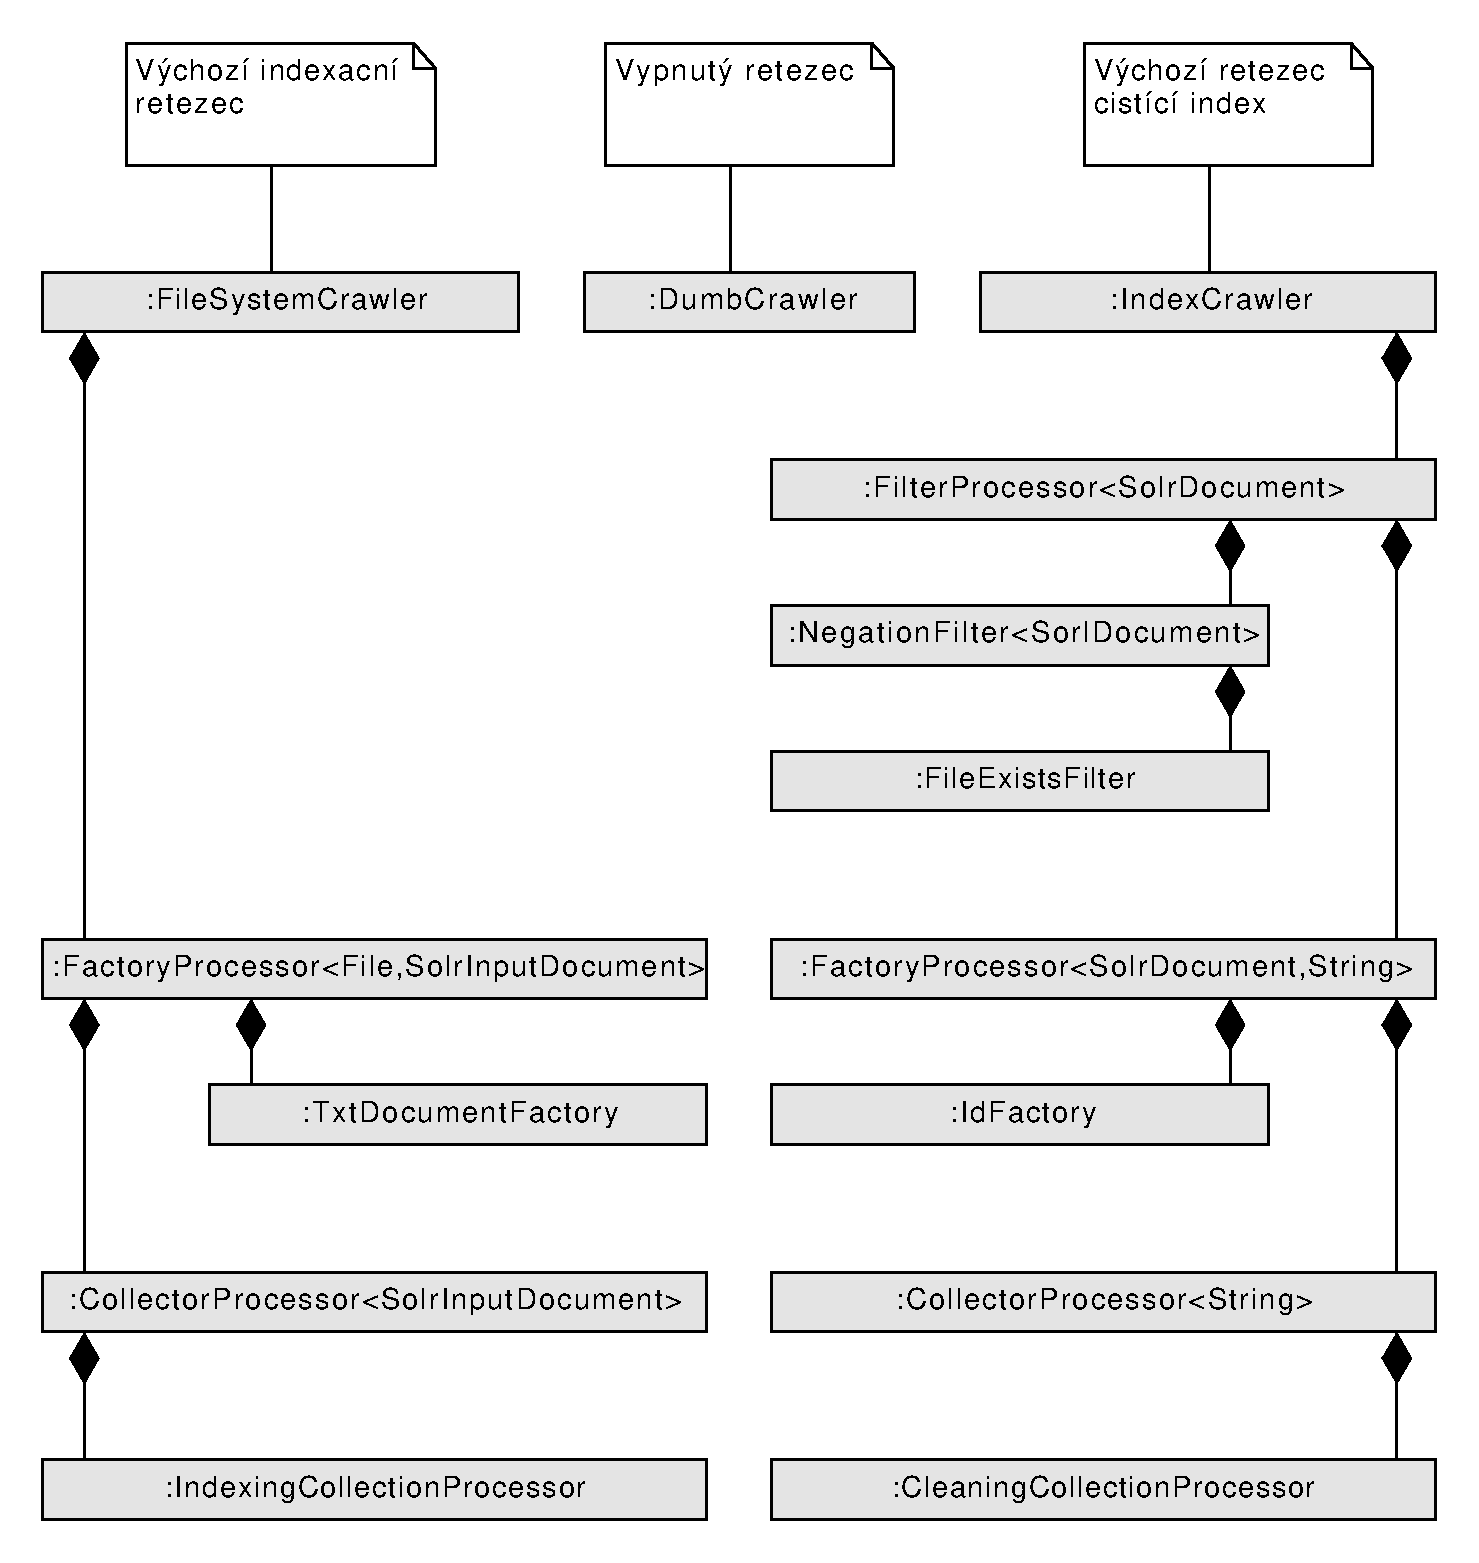
\includegraphics[width=13cm]{ProcessorChain}
\caption{Objektový model sestavených procesorových řetězů Crawleru}
\label{fig:ProcessorChain}
\end{center}
\end{figure}


\subsection{Sestavení}
Kompilace aplikace je nastavena tak, aby se vytvořil JAR soubor obsahující všechny knihovny, na kterých aplikace závisí. K~aplikaci jsem vytvořil skript pro prostředí Windows i~Linux, který zjednoduší její spouštění.

\section{Frontend}
Frontend podle pospaného návrhu sestává ze dvou statických HTML stránek oživených pomocí JavaScriptu. Pro usnadnění tvorby layoutu jsem využil CSS knihovny Bootstrap\cite{bootstrap}, která přináší jednotný a~přehledný vizuální styl a~definuje vizuální komponenty nad rámec prostého HTML.

Stránku jsem oživil pomocí JavaScriptové knihovny Angular.js\cite{angular}, která mi umožnila provázat backend v~podobě Solru s~HTML frontendem za použití služeb pro JSON komunikaci se serverem a~tzv. two way bindingu, mechanismu k~provázání HTML DOM s~JavaScriptovým modelem. Angular.js zastoupil i~původní JavaScriptovou knihovnu Bootstrapu, protože umožňuje definovat mnohem jednodušším způsobem skrývání komponent a~prvků v~návaznosti na události.

Oproti popsanému návrhu v~kapitole \ref{design_frontend} jsem opatřil prvky ikonami ze sady volně použitelných univerzálních ikon FontAwesome\cite{fontawesome}, které usnadní vizuální navigaci uživatele po stránce. Ikonami jsem nahradil i~původně zamýšlené zaškrtávací vstupní pole u~jednotlivých shluků. Použil jsem ikonu adresáře, kterou uživatelé znají a~která napoví, že položky znázorňují jisté skupiny dokumentů. Vybrané shluky se znázorní ikonou otevřeného adresáře. Číselné vyjádření počtu dokumentů ve shluku jsem umístil do komponenty \emph{badge}, kterou je zvykem na internetu používat k~tomuto účelu. Seznam shluků, do kterých patří dokumenty ve výsledcích, jsou umístěné ve vizuální komponentě \emph{label}, kterou je zvykem používat například pro zobrazení štítků u~položek. Výsledný layout lze vidět na obrázcích \ref{fig:ScreenSearcher} a~\ref{fig:ScreenDetail}.

Aplikace počítá s~nasazením aplikace Solr na stejném webovém serveru. Služby načítající data se přímo odkazují na request handlery \emph{/solr/searcher} a~\emph{/solr/detail} definované v~kapitole \ref{sorlconfig}, a~kromě toho získávají data o~dostupných indexech pomocí vnitřního handleru \emph{/solr/admin/cores}.

Při implementaci jsem dbal na to, aby web odpovídal běžným zvyklostem i~přesto, že je implementovaný v~JavaScriptu. Všechny změny stavu aplikace jsou proto promítány i~do adresního řádku. Díky tomu lze například zkopírováním adresy odkazovat na konkrétní výsledky vyhledávání, využívat funkcí zpět a~vpřed v~historii prohlížeče, či otevírat odkazy v~novém okně pomocí běžných prostředků prohlížeče. Využívám k~tomu standardní \emph{Angular.js} službu \emph{Route}, která zprostředkovává parsování i~změny informací v~adresním řádku.

Aby mohl být frontend nasazen do servlet containeru, umístil jsem všechny statické soubory do adresáře \emph{webapp} webové aplikace a~vytvořil \emph{HttpServlet} pojmenovaný \emph{ViewFile}, jehož jedinou funkcí je odeslat jako odpověď na požadavek obsah souboru. V~konfiguračním souboru \emph{WEB-INF/web.xml} jsem servlet zaregistroval a~namapoval na něj všechny url adresy. 

Výsledná aplikace se kompiluje jako WAR soubor, který je možné nasadit do servlet containeru.

\begin{verbatim}
<servlet>
  <servlet-name>ViewFile</servlet-name>
  <servlet-class>
    cz.cvut.skorpste.dip.frontend.ViewFile
  </servlet-class>
</servlet>

<servlet-mapping>
  <servlet-name>ViewFile</servlet-name>
  <url-pattern>/*</url-pattern>
</servlet-mapping>
\end{verbatim}

\section{Jetty}
Posledním krokem v~rámci implementace řešení byla konfigurace serveru Jetty. Použil jsem instalaci distribuovanou se Solrem. Port serveru jsem nastavil na 8080 místo standardního 80, abych minimalizoval kolizi s~jiným webovým serverem, a~aby pro běh aplikace nebyla zapotřebí práva správce. Do aplikace jsem přidal webovou aplikaci \emph{frontend} a~nastavil \emph{contextPath} na kořenový adresář serveru. Pro usnadnění spouštění aplikace jsem napsal krátké scripty pro prostředí Linux i~Windows.

\begin{figure}[h]
\begin{center}
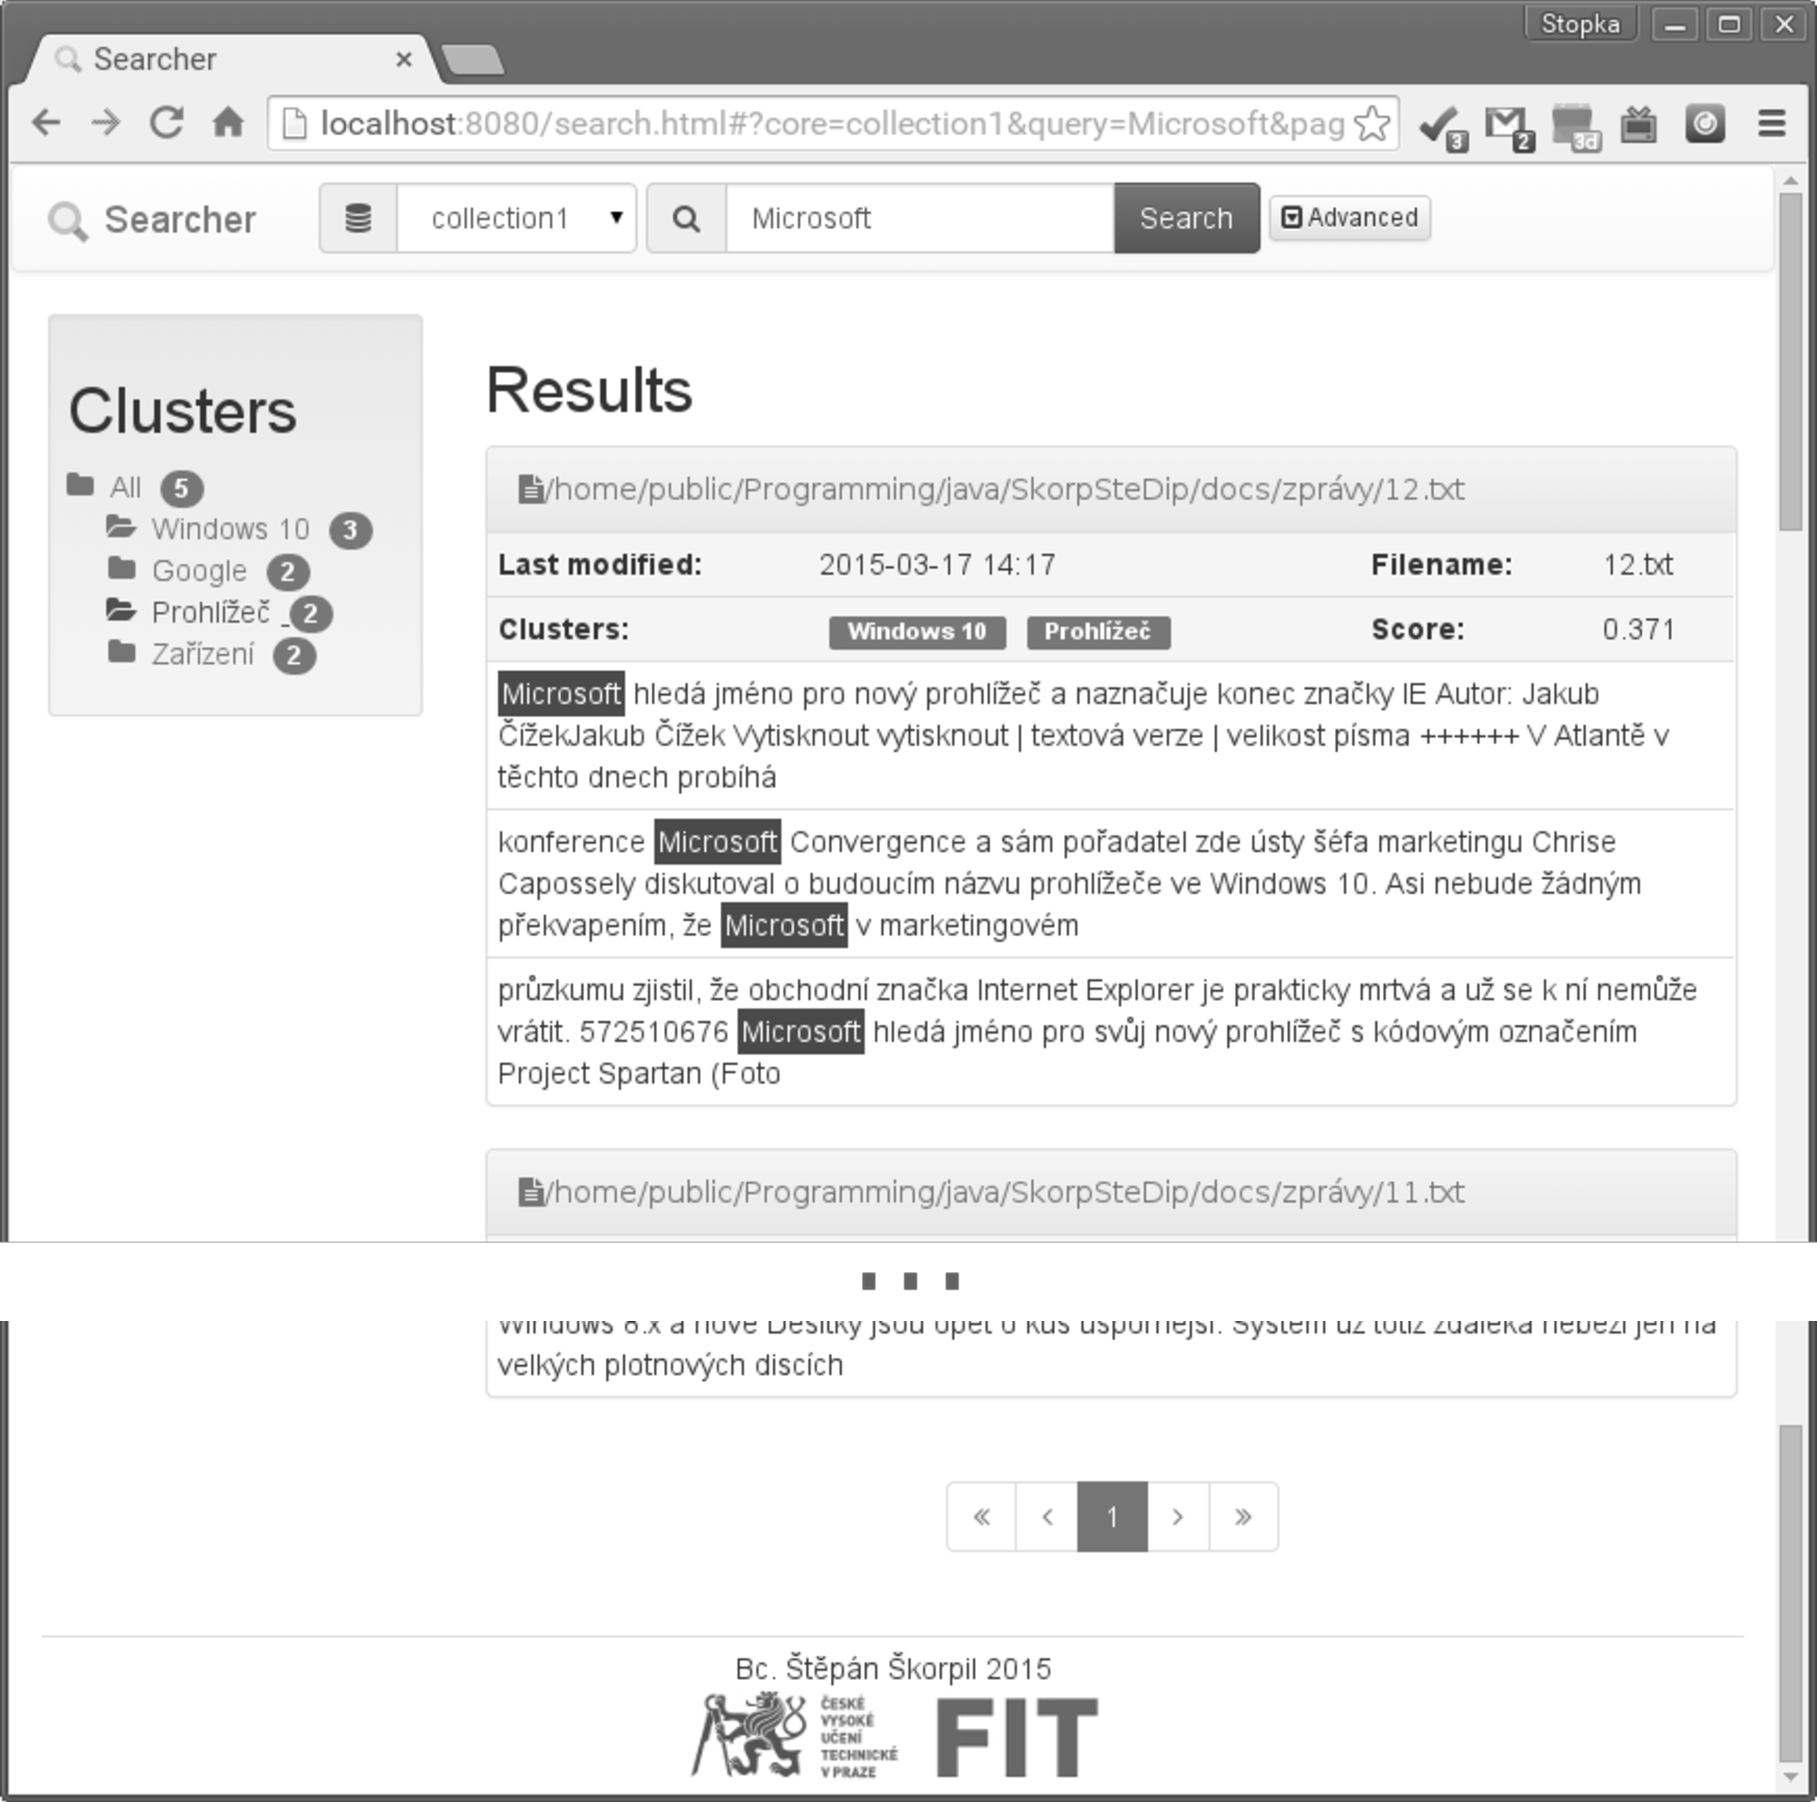
\includegraphics[width=13cm]{ScreenSearcher}
\caption{Snímek UI (Vyhledávač)}
\label{fig:ScreenSearcher}
\end{center}
\end{figure}

\begin{figure}[h]
\begin{center}
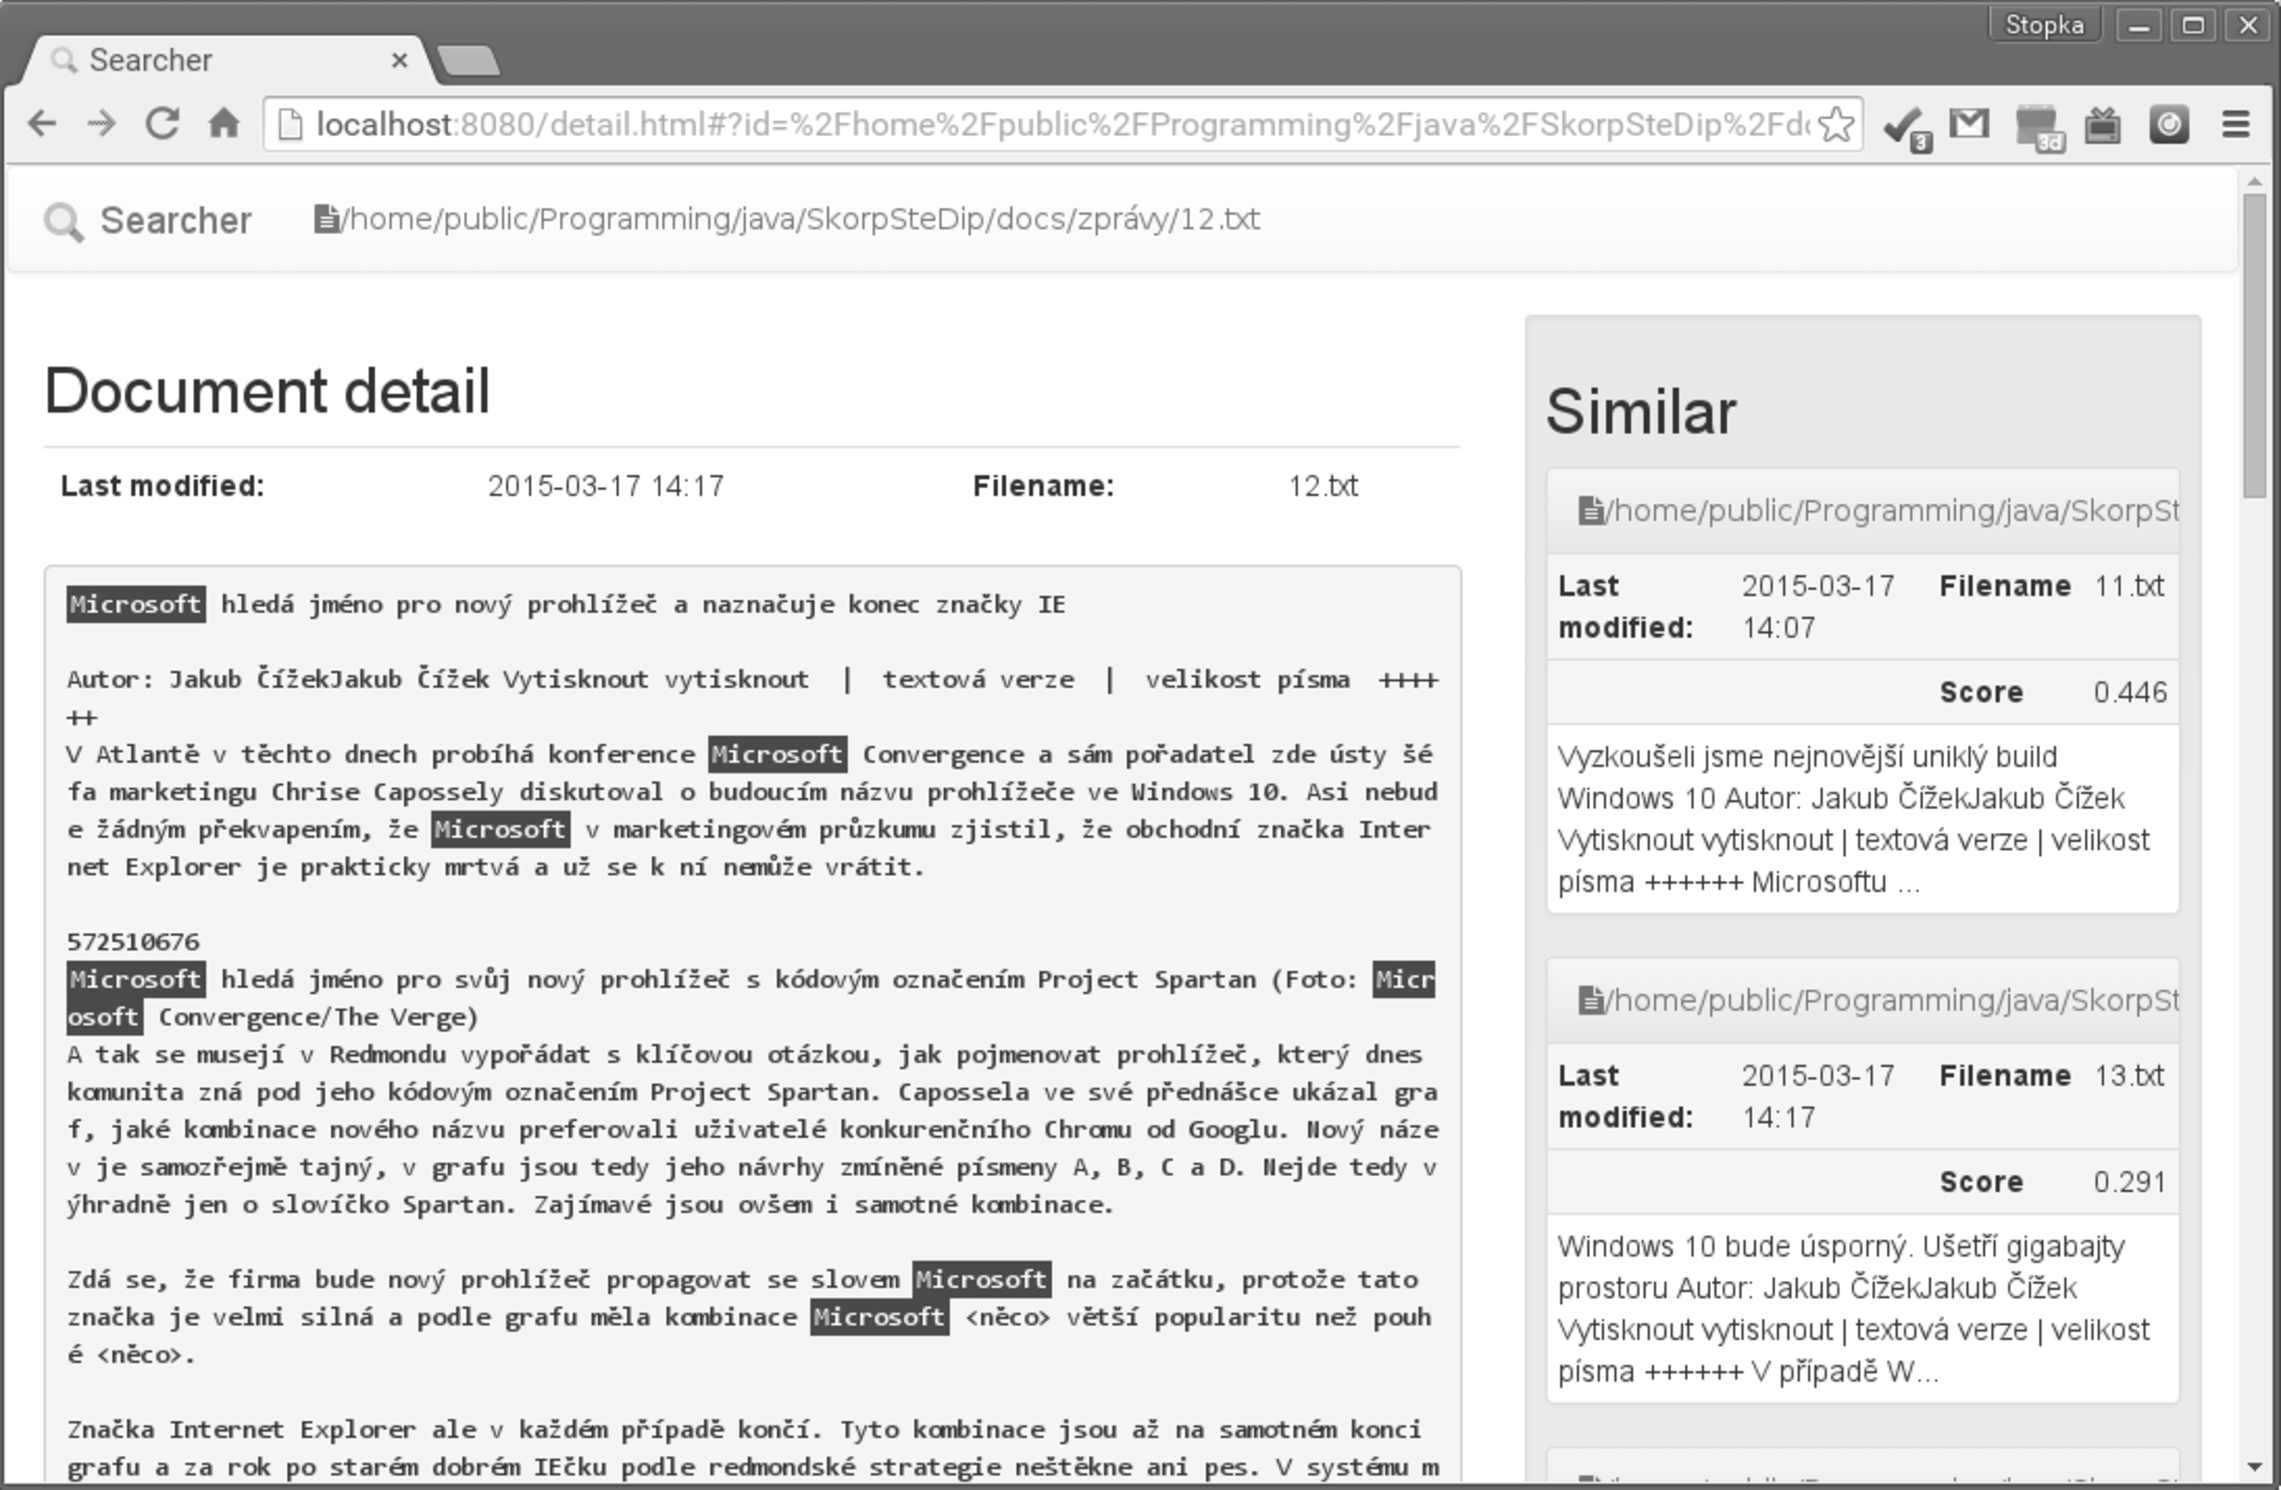
\includegraphics[width=13cm]{ScreenDetail}
\caption{Snímek UI (Detail dokumentu)}
\label{fig:ScreenDetail}
\end{center}
\end{figure}